\section{OpenCADC}

\textit{This research used the facilities of the Canadian Astronomy Data Centre operated 
by the National Research Council of Canada with the support of the Canadian Space Agency}.\\

OpenCADC (Canadian Astronomy Data Center) is a Virtual Observatory, used in ALMA Science Archive (for this reason is included in this chapter) tool which comprises several projects \footnote{We do not enumerate all of them here, for a full list, go to \url{https://code.google.com/p/opencadc/source/browse}}:

\subsection{UWS}

The Universal Worker Service (UWS) pattern defines how to build asynchronous (the client does not wait for each request to be fulfilled; if the client disconnects from the service then the activity is not aborted), stateful (the service remembers results of a previous activity), job-oriented (the rules for setting and arranging the parameters for a job is called Job Description Language- JDL) services.

\begin{figure}[H]
\centering
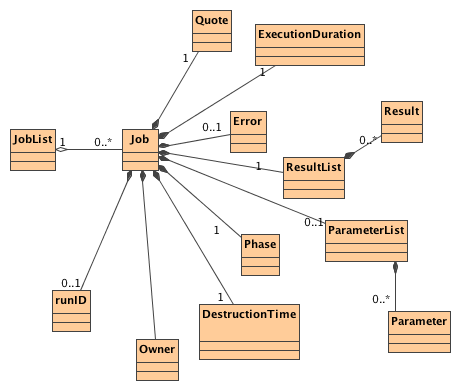
\includegraphics[width=11cm,height=8cm]{images/Class_Diagram__UWS__UWSObjects.png}\\
\caption{UWS Objects in class diagram}
\end{figure}

When the execution starts, the job is seen as a state machine which can adopt several states. The phases are the following:

\begin{itemize}

\item 
    PENDING: the job is accepted but not committed for execution by the client.
\item
    QUEUED: the job is committed for execution by the client but the service has not yet assigned it to a processor.
\item
    EXECUTING: the job has been assigned to a processor and the results can be produced at any time during this phase.
\item
    COMPLETED: execution is over and the user can collect the results.
\item
    ERROR: the job failed to complete.
\item
    ABORTED: the job has been stopped by the user or by the system.
\item
    UNKNOWN: the job is in an unknown state.
\item
    HELD: the job is pending execution.
\item
    SUSPENDED: The job has been suspended by the system during execution. This might be because of temporary lack of resource. Similar to aborted but in this state the UWS will automatically resume the when resource are available again.

\end{itemize}

% \begin{lstlisting}
% public enum ExecutionPhase
% {
%     PENDING("PENDING"),
%     QUEUED("QUEUED"),
%     EXECUTING("EXECUTING"),
%     COMPLETED("COMPLETED"),
%     ERROR("ERROR"),
%     UNKNOWN("UNKNOWN"),
%     HELD("HELD"),
%     SUSPENDED("SUSPENDED"),
%     ABORTED("ABORTED");
% 
%     private String value;
% 
%     private ExecutionPhase(String value) { this.value = value; }
% 
%     public static ExecutionPhase toValue(String s)
%     {
%         for (ExecutionPhase d : values())
%             if (d.value.equals(s))
%                 return d;
%         throw new IllegalArgumentException("invalid value: " + s);
%     }
% 
%     public String getValue() { return value; }
% }
% 
% \end{lstlisting}


\begin{figure}[H]
\centering
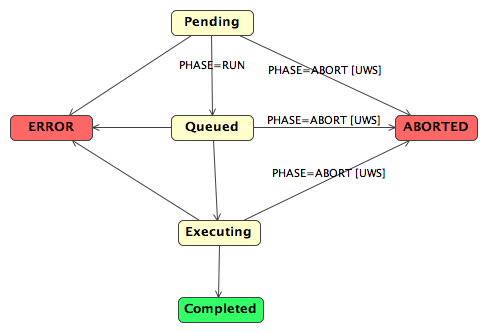
\includegraphics[width=11cm,height=8cm]{images/UWSStates.png}\\
\caption{Universal Worker Server Job states}
\end{figure}

Now, we make a subtle description of the structure of the code relating UWS in OpenCADC (the cadcUWS Library), the section of the code provides Job class and plugin architecture, servlet with UWS async and sync behaviour.

\subsubsection{JobManager}

Responsible for job control.

\subsubsection{JobPersistence}

In charge of storing and retrieving Job state.

\subsubsection{JobExecutor}

It executes every job in separated threads.

\subsubsection{JobRunner}

The code that actually executes the job.


\subsection{cadcTAP Library}

The cadcTAP library is responsible of async and sync queries, where QueryRunner implements JobRunner. It also contains TAP\_SCHEMA DDL statements and is used by query parser to validate table and column usage.

\subsubsection{TapQuery Interface}

It has a separate implementation for each LANG (e.g. $LANG = ADQL$) specified and processess the query to local SQL.

\subsubsection{SqlQuery}

When code states $LANG=SQL$, it implements TapQuery and fully navigates it ($FROM, WHERE$ and $HAVING$ clauses).

\subsubsection{AdqlQuery}

Same as before when $LANG=ADQL$.

\subsubsection{Plugins}

\begin{itemize}
\item UploadManager
\item TableWriter
\item FileStore
\end{itemize}


\subsubsection{QueryRunner}

It implements JobRunner and sets Job state, find DataSource and uses TapSchema, UploadManager, TapQuery and TableWriter.

